 \section{Asignación Clásica y Alternativa}
 Hasta ahora hemos visto la \textbf{conveción clásica de D-H} para asignar los índices de marcos de referencia y parámetros a una cadena cinemática abierta simple. Sin embargo, también existe la \textbf{conveción modificada de D-H} que utilizan libros como \textit{Introducción a la Robótica: Mecánica y Control (3.ª edición)}[4]. Cabe destacar que el conteo (primer, segundo, ...) e indexado (0, 1, ...) de los eslabones y articulaciones es igual en ambas conveciones.

 \subsection{Convención clásica D-H}
Se asignan los marcos de referencia y los parámetros como lo hemos visto hasta ahora. Es decir, el índice $i$ de un eslabón $l_i$ se utiliza para los índices del sistema de coordenadas de la articulación $i+1$. Se dice que los parámetros de esta conveción clásica son \textbf{parámetros distales}. En la figura~\ref{fig:convencion-clasica} se muestra esta convencion clásica.

\begin{figure}[H]
        \centering
        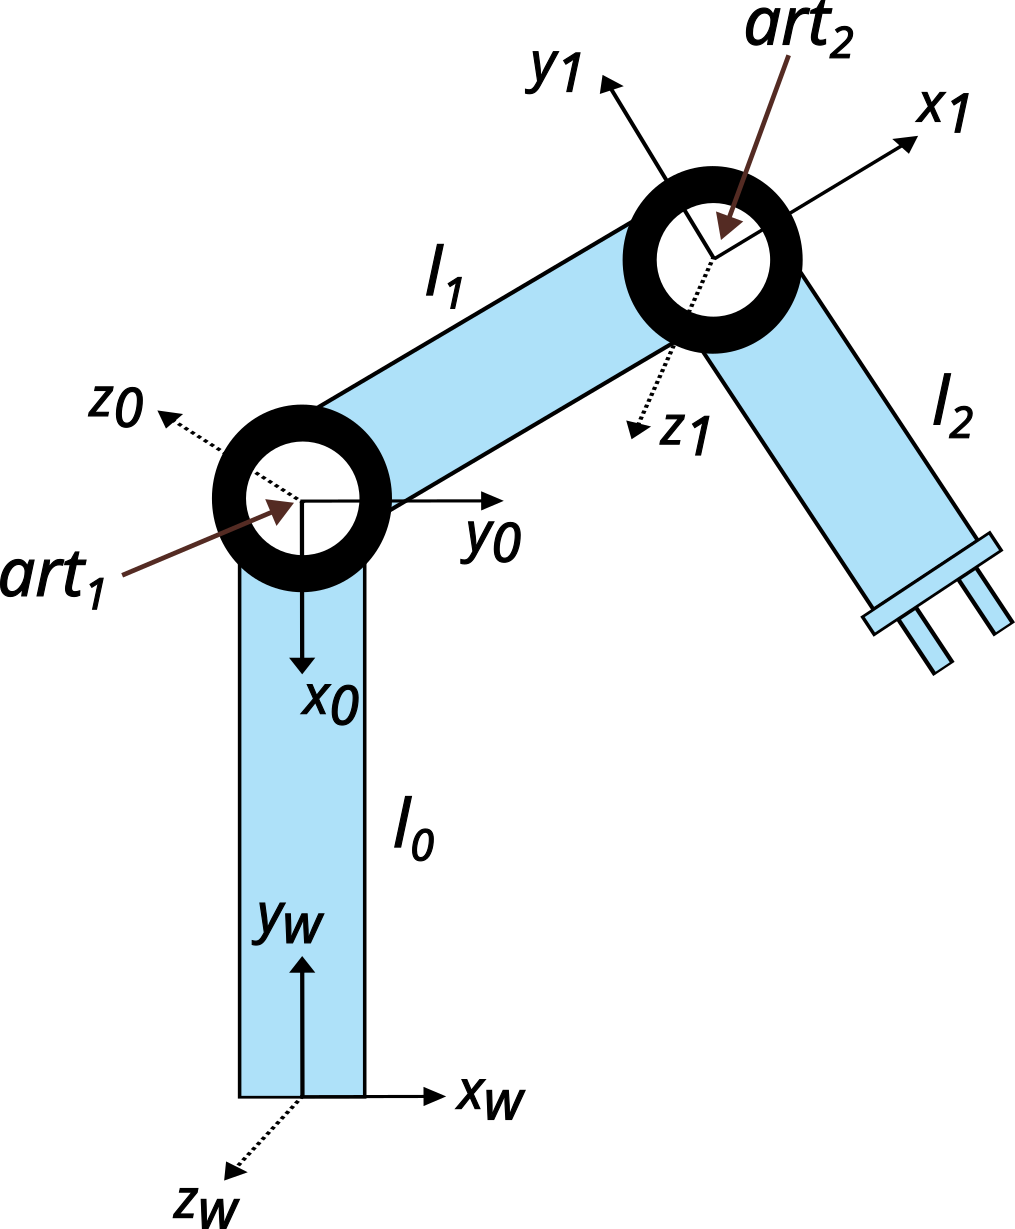
\includegraphics[width=0.45\textwidth]{imagenes/convencion-clasica.png}
        \caption{Convención clásica D-H.}
        \label{fig:convencion-clasica}
\end{figure}

 \subsection{Convención modificada o alternativa D-H}
 En esta convención, el índice $i$ de un eslabón $l_i$ se utiliza para los índices del sistema de coordenadas de la articulación $i$. Se dice que los parámetros de este convención modificada son \textbf{parámetros proximales}. En la figura~\ref{fig:convencion-modificada} se muestra esta convencion modificada.

 \begin{figure}[H]
        \centering
        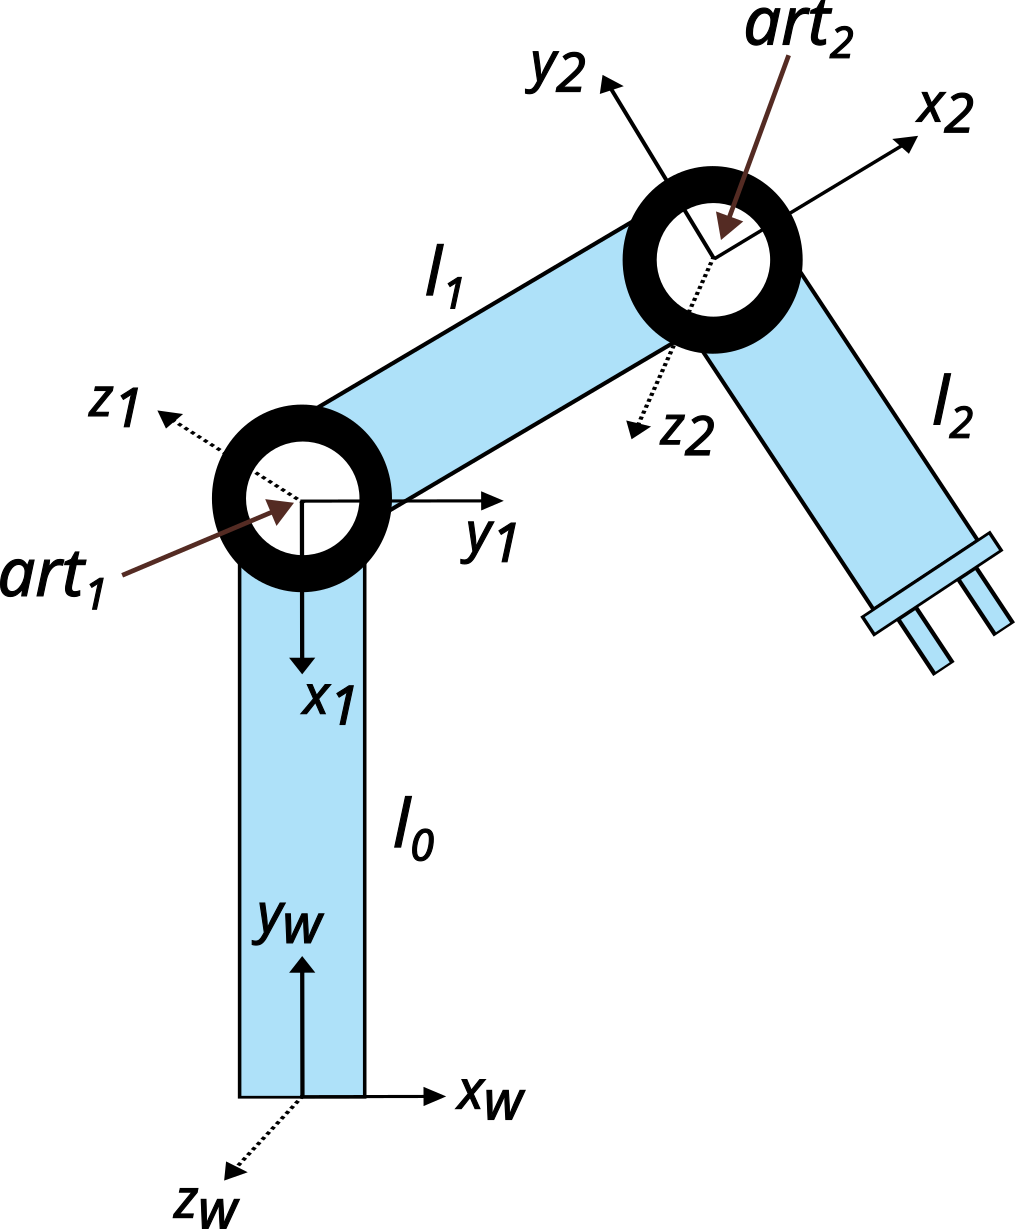
\includegraphics[width=0.45\textwidth]{imagenes/convencion-modificada.png}
        \caption{Convención modificada D-H.}
        \label{fig:convencion-modificada}
\end{figure}


